\section{Basic Document Structure}

The basic document structure in \LaTeX{} looks like the following figure.

\begin{myTEXEX}{}
%
% Preamble
%

\documentclass[]{myHOWTO-V1}

\title{MyDocument}
\version{1.00}
\author{Norbert EHART}
\date{\today}

%
% Body
%

\begin{document}
	
\selectlanguage{english}

\maketitle
\tableofcontents
\listoffigures

\input{SomeFileToInclude.tex}

\printbibliography

\end{document}
\end{myTEXEX}

In the preamble, the document class has to be specified and some variables. Anything else should not be in the preamble, because layout and formatting is defined in the document class. There are a few exceptions, which we will cover later. The variables are mandatory and will be used to create the title page later.

The body starts with \Verb|\begin{document}| and ends with \Verb|\end{document}|. The content of the document is placed between these two commands.

The first thing that needs to be defined in the body of the document is the language. I would recommend defining it anyway, even a default language of English is specified. If the document is written in German, you will have to enter \Verb|\selectlanguage{ngerman}| instead of \Verb|\selectlanguage{english}|. It is important that the correct language is selected. Without this configuration, hyphenation may be incorrect. Also, the language-specific commands in the document may not be translated (table of contents, table of figures, bibliography, etc.).

You can create a predefined title page with \Verb|\maketitle|. For this purpose a new command \Verb|\version{}| has been introduced to display the document version.  All used variables \Verb|\title{}|, \Verb|\version{}|, \Verb|\author{}| and \Verb|\date{}| are mandatory in order to use the \Verb|\maketitle| command.

\centering
\begin{myFIG}{}
	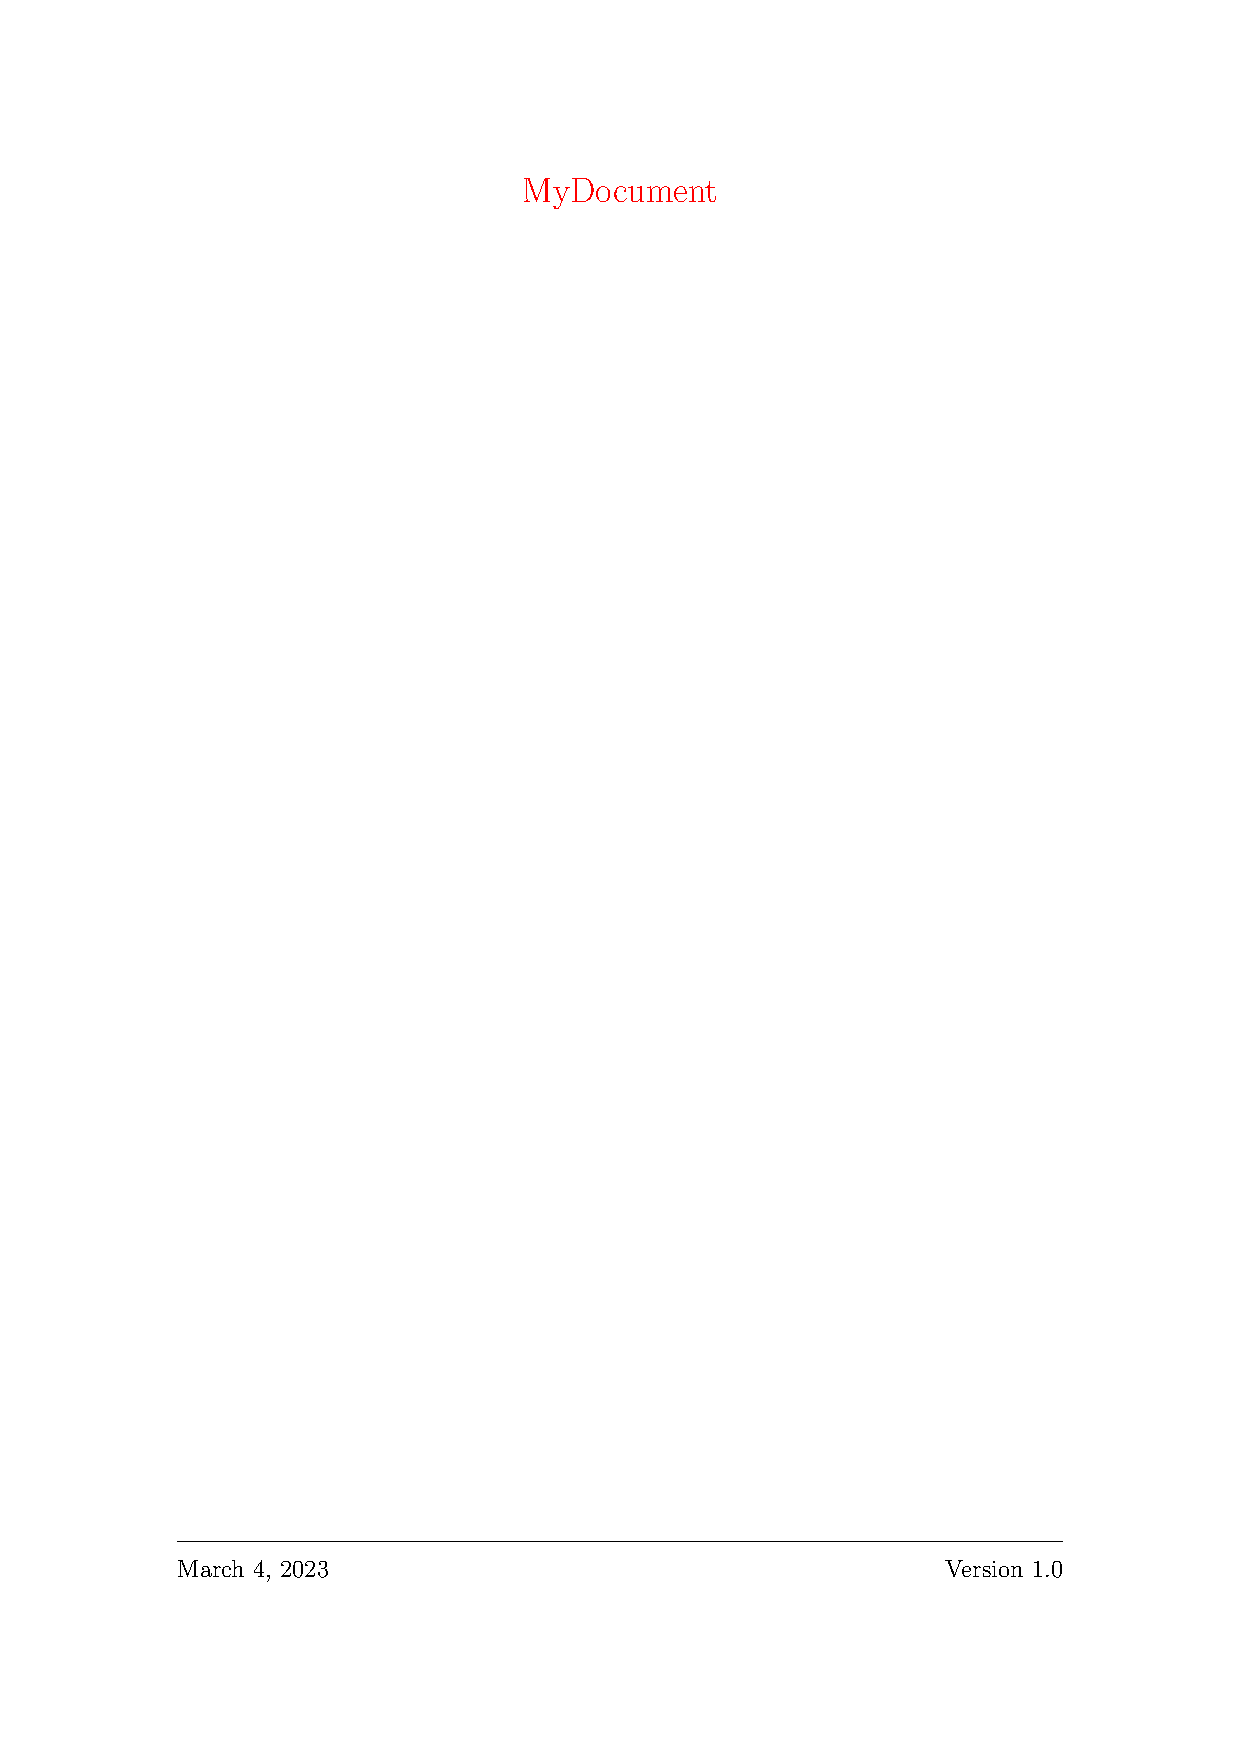
\includegraphics[page=1,scale=0.25]{examples/zz_bsp_file_CoverPage.pdf}
\end{myFIG}
\quad
\begin{myFIG}{}
	\includegraphics[page=2,scale=0.25]{examples/zz_bsp_file_CoverPage.pdf}
\end{myFIG}

\justifying

The \Verb|\input{SomeFileToInclude.tex}| command makes \LaTeX{} to process the content of the given file basically the same way as if it would be written at the same place as \Verb|\input{SomeFileToInclude.tex}|. Mentionable properties of \Verb|\input{}| are:

\begin{itemize}
	\item You can use \Verb|\input{}| basically everywhere with any content.
	\item You can use \Verb|\input{}| inside a file which is read using \Verb|\input{}|.
\end{itemize}

The bibliography is created automatically from the file \emph{references.bib} with the command \Verb|\printbibliography|. The filename is mandatory and can not be changed. The file \emph{references.bib} looks something like this.

\begin{myFILE}{}
@misc{geometry2020,
	author = {{Hideo Umeki}},
	title = {{The geometry package}},
	year = {2020}, 
	howpublished = {\url{https://mirror.at/example}},
}
\end{myFILE}

But be careful, if the bibliography is instantly visible in the PDF or not, depends on the editor. One editor makes the bibliography immediately during the compiling process, the other must first generate a \emph{bbl} file using \emph{biblatex}. In e.g. \emph{\TeX studio}, a \emph{bbl} must be generated using biblatex before it is visible in the PDF.

\centering
\begin{myFIG}{}
	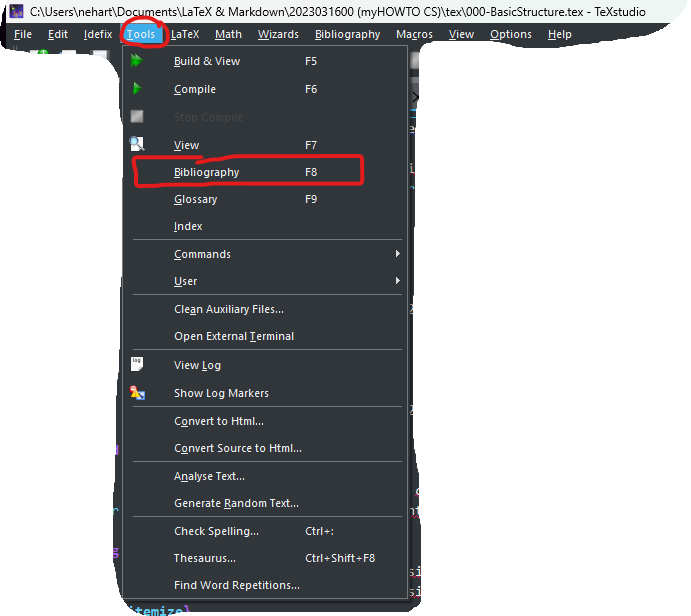
\includegraphics[scale=0.4]{pictures/Using_biblatex_in_TeXstudio.png}
\end{myFIG}

\justifying

It should also be mentioned that by default all entries in \emph{references.bib} are inserted into the list of figures

For headlines you can use the commands \Verb|\section{}|, \Verb|\subsection{}| and \\ \Verb|\subsubsection{}|. It will appear in the PDF file as displayed in the following figure.

\centering
\begin{myFIG}{}
	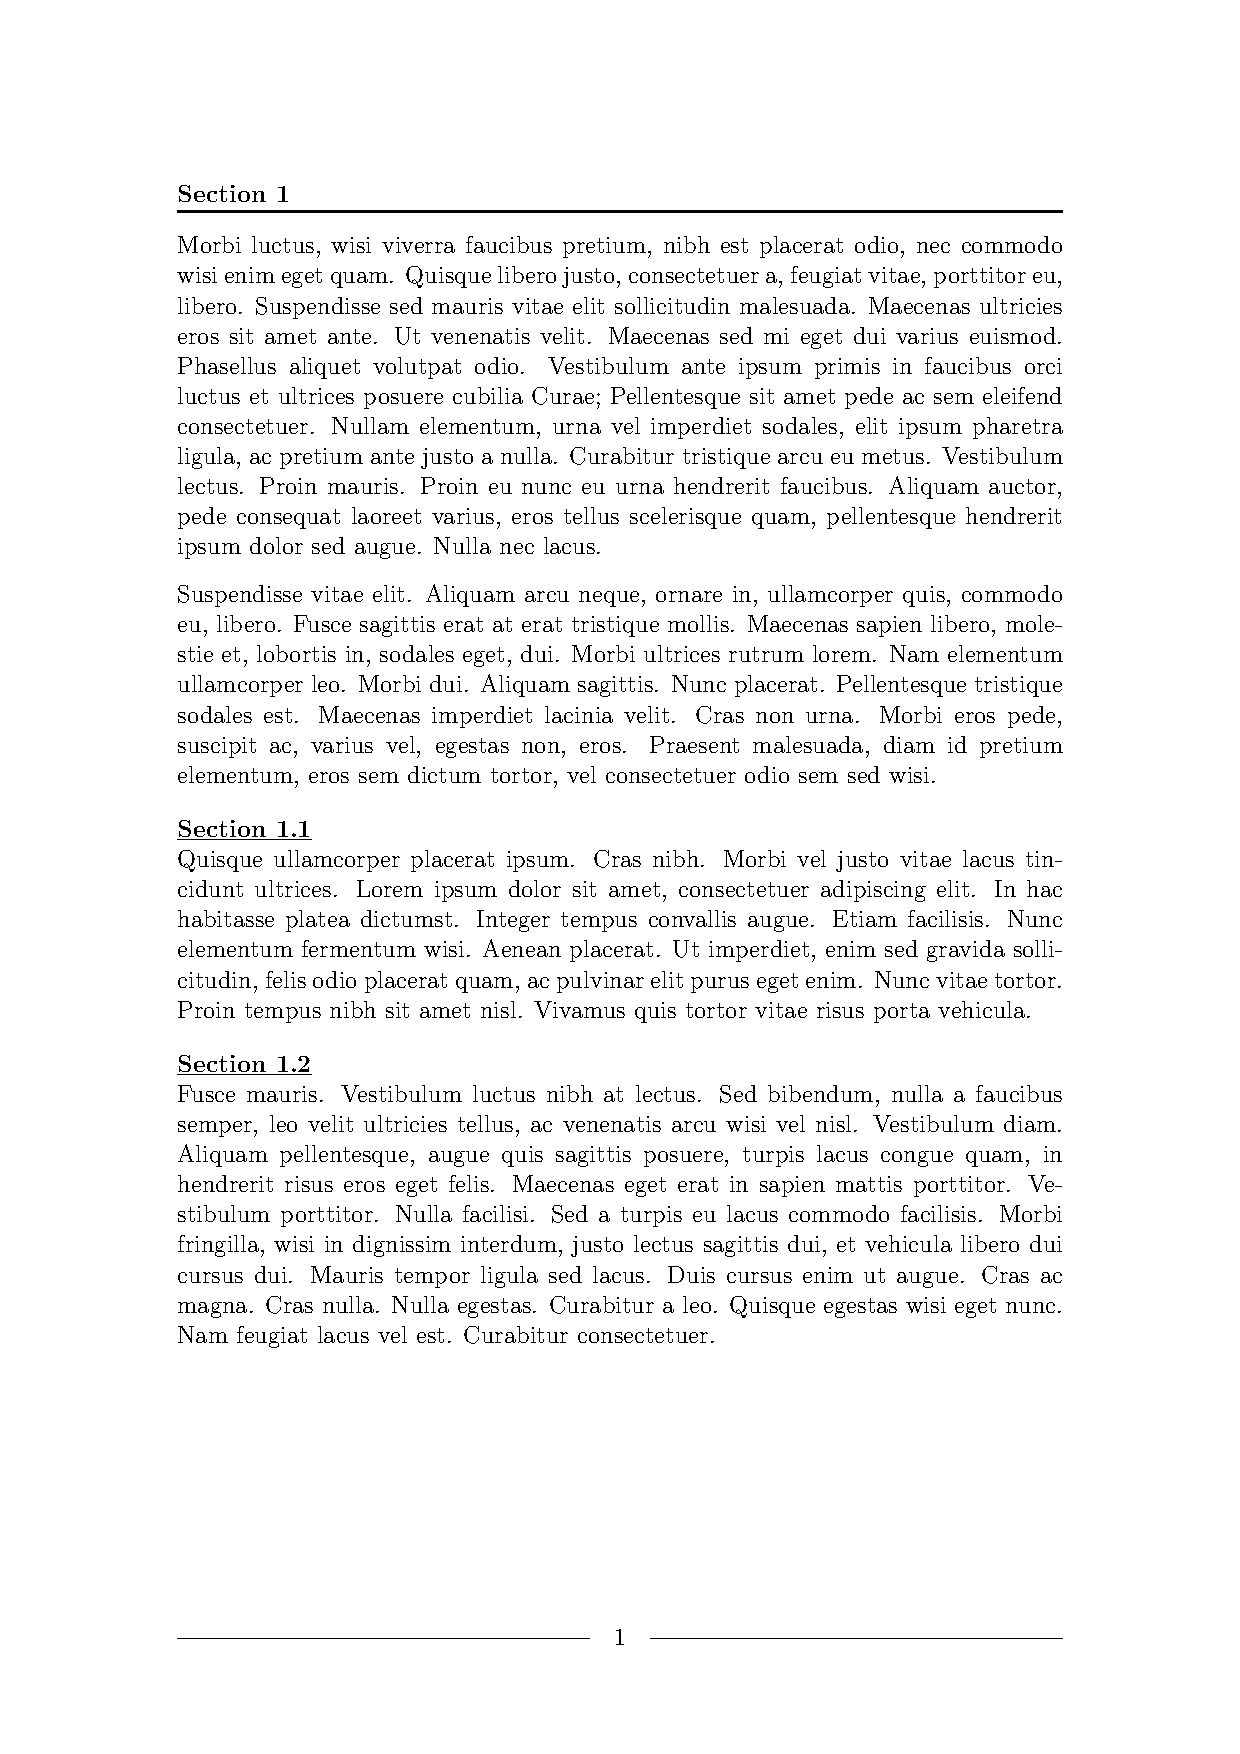
\includegraphics[page=1,scale=0.22]{examples/zz_bsp_file_Headlines.pdf}
\end{myFIG}
\quad
\begin{myFIG}{}
	\includegraphics[page=2,scale=0.22]{examples/zz_bsp_file_Headlines.pdf}
\end{myFIG}

\justifying

The \Verb|\tableofcontents| command must be used to print the table of contents. Only \Verb|\section{}| will appear in the table of contents. Headlines created with \Verb|\subsection{}| and \Verb|\subsubsection{}| will not be shown in the table of contents. 

In order to create the list of figures, the \Verb|\listoffigures| command is used.

The following image shows how this looks.

\centering
\begin{myFIG}{}
	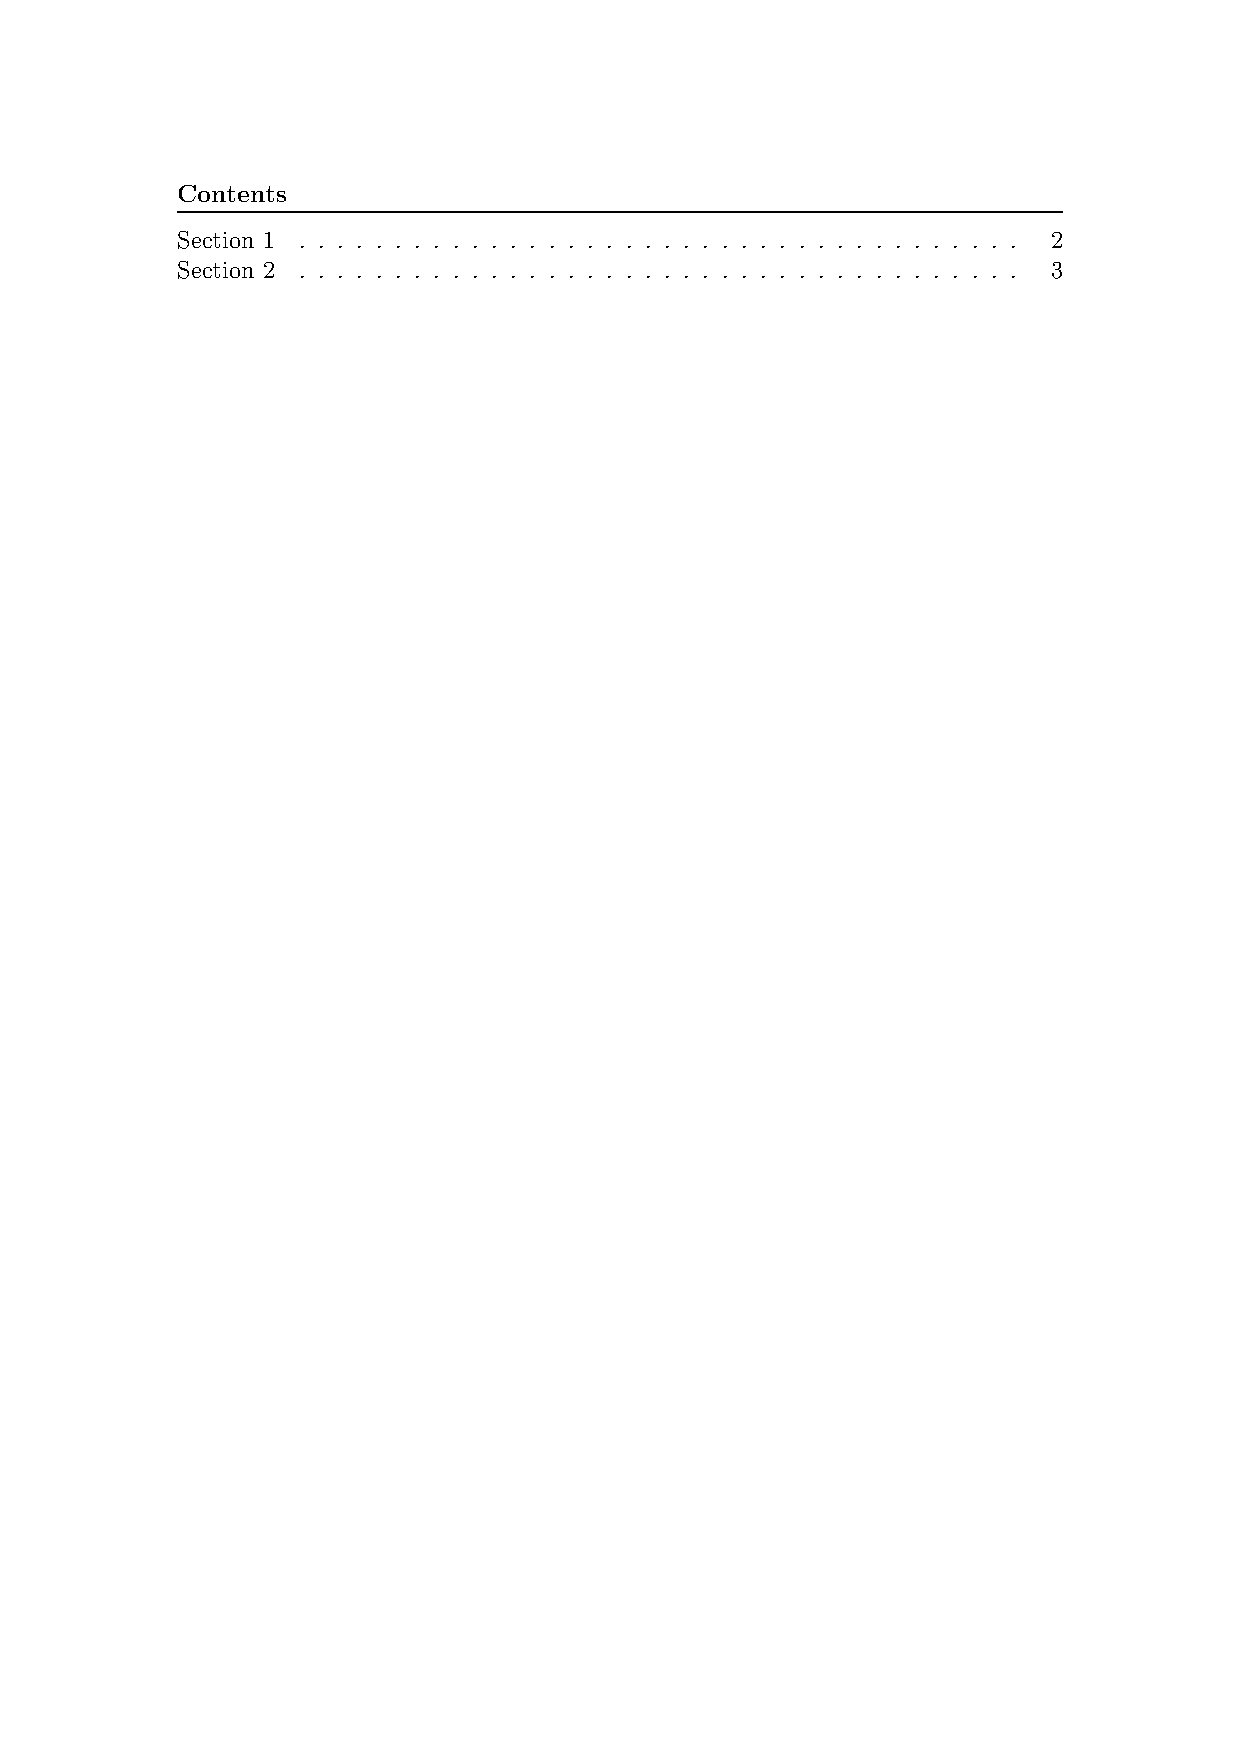
\includegraphics[page=1,scale=0.24]{examples/zz_bsp_file_TOC.pdf}
\end{myFIG}
\quad
\begin{myFIG}{}
	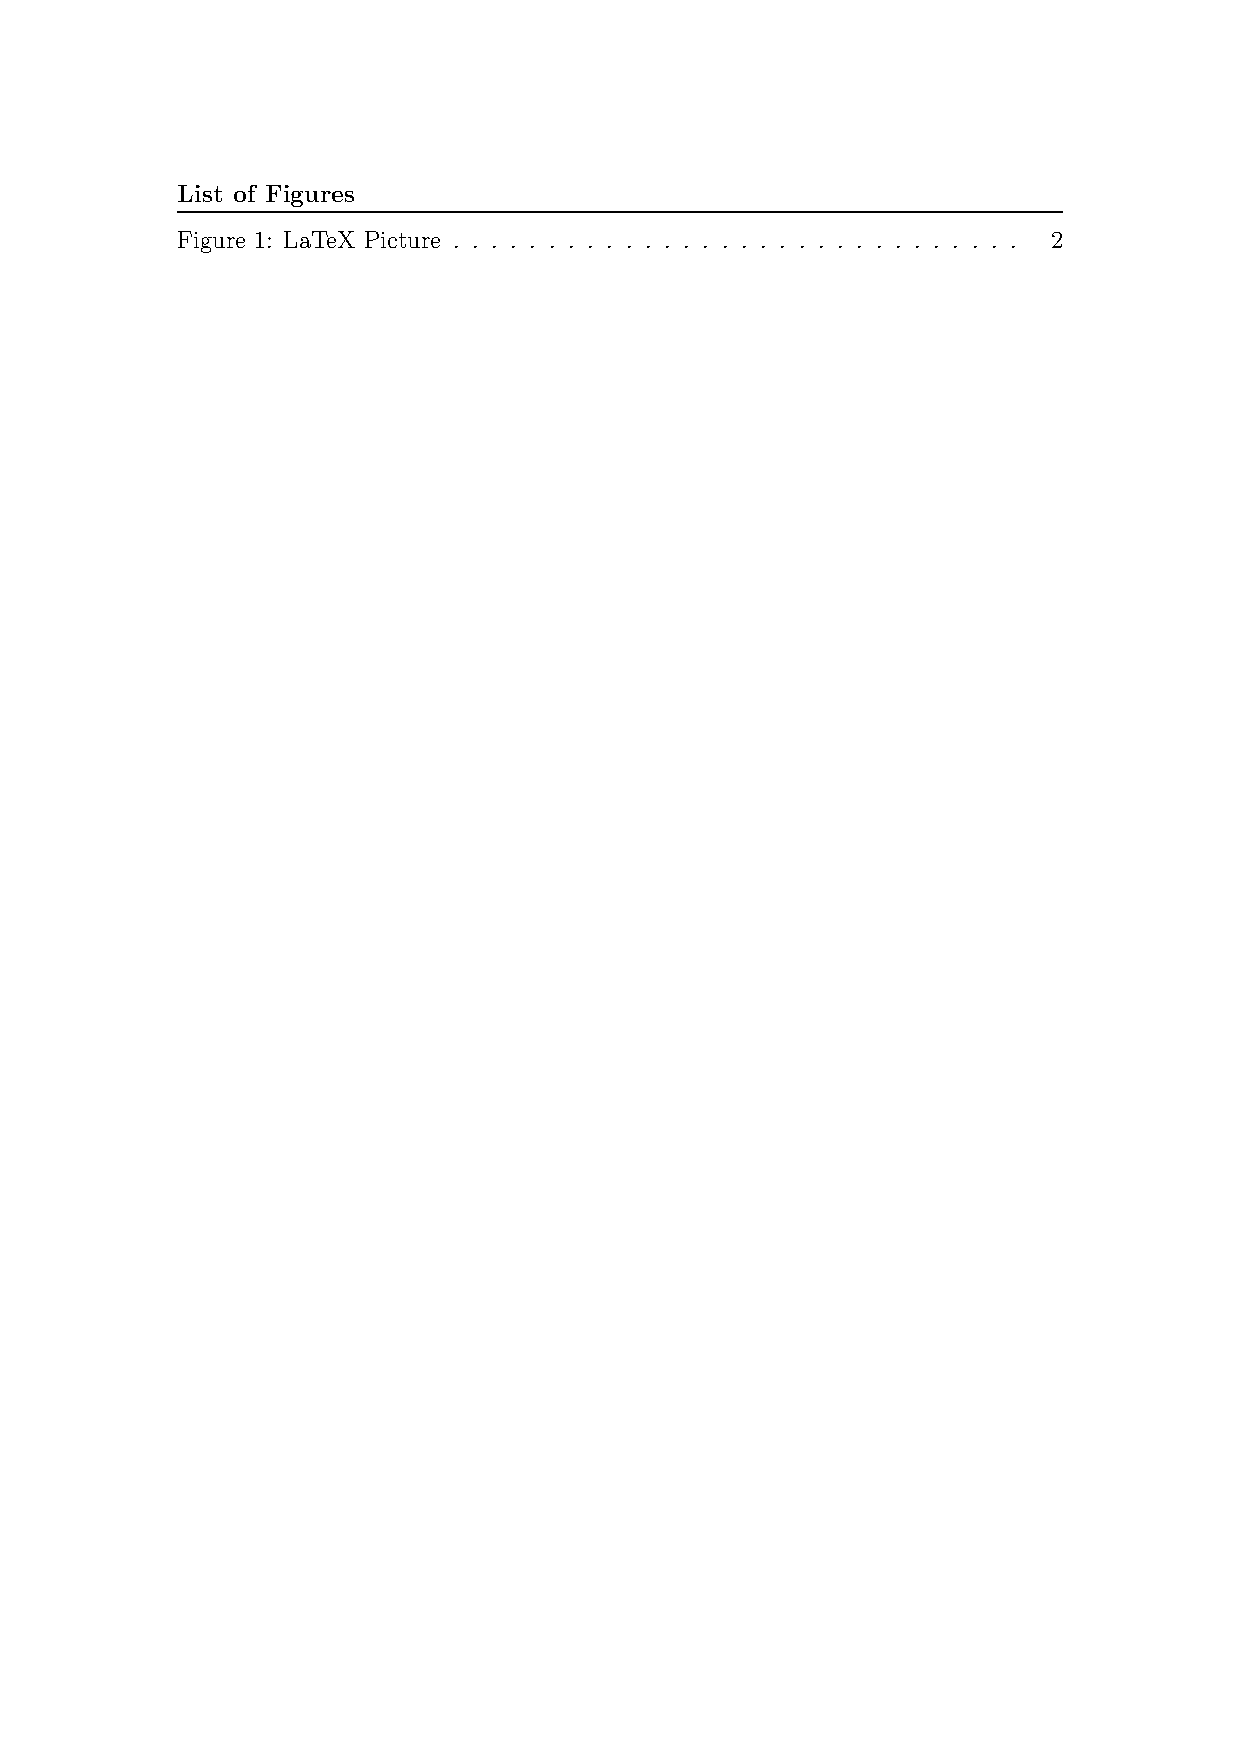
\includegraphics[page=1,scale=0.24]{examples/zz_bsp_file_LOF.pdf}
\end{myFIG}

\justifying

The standard text can be written in LaTeX simply between the \Verb|\begin{document}| and \Verb|\end{document}| environment without any commands. Two line breaks in a row (equivalent to a blank line) will create a new paragraph. If you only want to end the line without starting a new paragraph, you have to use \Verb|\\|. Hyphenation shouldn't be done by yourself in any case, this is done by \LaTeX.